\documentclass[a4paper,12pt]{article} 


\usepackage[T2A]{fontenc}			
\usepackage[utf8]{inputenc}			
\usepackage[english,russian]{babel}	

\usepackage{graphicx, scalerel}    
\usepackage{wrapfig}               
\usepackage[14pt]{extsizes}        
\usepackage[warn]{mathtext}       
\usepackage{indentfirst}      
\usepackage[margin = 25mm]{geometry}
\usepackage[table,xcdraw]{xcolor} 
\usepackage{amsmath,amsfonts,amssymb,amsthm,mathtools}
\usepackage{wasysym}                
\usepackage{upgreek}                
\usepackage{caption}
\usepackage{multirow}
\captionsetup{labelsep=period}
\usepackage[font=small,labelfont=bf]{caption}
\usepackage{gensymb}
\usepackage[unicode, pdftex]{hyperref}
\usepackage{tikz}
\usetikzlibrary{positioning}
\usepackage{fancyhdr}
\pagestyle{fancy}
\setlength\fboxsep{3pt} % Отступ рамки \fbox{} от рисунка
\setlength\fboxrule{1pt} % Толщина линий рамки \fbox{}
\newcommand{\tocsection}[1]{\section*{#1} \addcontentsline{toc}{section}{#1}}
\newcommand{\tocsubsection}[1]{\subsection*{#1} \addcontentsline{toc}{subsection}{#1}}
\renewcommand{\cftsecleader}{\cftdotfill{\cftdotsep}}

\begin{document}
		\newcommand{\HRule}{\rule{\linewidth}{0.7mm}} % Defines a new command for the horizontal lines, change thickness here

\begin{center}
	\large\textbf{Московский Физико-Технический Институт}\\
	\large\textbf{(государственный университет)}
	
	\vfill
	

	
	\Large Вычислительная математика
	%----------------------------------------------------------------------------------------
	%	TITLE SECTION
	%----------------------------------------------------------------------------------------
	
	\HRule
	\\[0.4cm]
	{ \huge \bfseries Лабораторная работа №9}
	\\[0.4cm] % Title of your document
	\HRule
	\\[0.5cm]
	
	\ \\
	\textbf{\large Автор:} \\	
	\large Овсянников Михаил Б01-008\\
	\vfill
	\hspace*{-0.8 cm}
\includegraphics[width=100 pt]{./Include/frkt_logo.pdf}\\
	\large Долгопрудный, 2023
\end{center}

\thispagestyle{empty}

\newpage
\setcounter{page}{2}
\fancyfoot[c]{\thepage}
\fancyhead[L] {Лабораторная работа №9}
\fancyhead[R]{}

		\tableofcontents
		\newpage
		
		\tocsection{Цель}
		Познакомиться с различными способами интерполяции, реализовать их и провести сравнение, сопоставить полученные значения с действительными и оценить ошибки.

		\tocsection{Теоретические сведения}
		\tocsubsection{Общая задача}
		 
		Пускай у нас есть набор данных зависимости одной величины от другой. Скажем, одна величина таблично задана от другой.
		\begin{table}[h!]
			\centering
				\begin{tabular}{|c|c|c|c|c|c|c|}
					\hline
					$x$    & $x_0$ & $x_1$ & $x_2$ & $\ldots$ & $x_{n-1}$ & $x_n$ \\ \hline
					$f(x)$ & $f_0$ & $f_1$ & $f_2$ & $\ldots$ & $f_{n-1}$ & $f_n$ \\ \hline
				\end{tabular}
			\caption{Таблично заданная функция}
		\end{table}
	
		Наша задача -- найти значения функции в точках, не указанных в таблице, то есть произвести интерполяцию, если говорить о точках между $x_1$ и $x_n$, и экстраполяцию в противном случае.
		
		Для этого всего применяются различные методы. В частности, используемые в данной работе многочлен Ньютона и сплайн-интерполяция. Остановимся на них поподробнее и рассмотрим их построение.
		
		\tocsubsection{Многочлен Ньютона}
		Это метод интерполяции, при котором искомая функция приближается многочленом степени $n$, где $n \leqslant N - 1$, $N$ -- количество точек в таблице. Причем все эти точки предполагаются попарно различными.
		
		Описание алгоритма построения состоит в следующем. Сначала посчитаем так называемые разделенные разности $b_k$. Для простоты будем предполагать, что используется вся таблица функции, хотя все следующее применимо и к определенному участку таблицы для интерполяции функции лишь по нескольким точкам из таблицы.
		
		Нулевая разделенная разность $b_0$ по определению есть значение функции в точке $x_i$, равное $f(x_i)$. Обозначим значения разделенных разностей для $b_{j-i}$ между точками $x_i$ и $x_j$, где $i < j$ как $f(x_i, x_{i+1}, \ldots, x_j)$. Они определяются рекурсивно:
		\begin{equation*}
			f(x_i, x_{i+1}, \ldots, x_{j-1}, x_j) = \frac{f(x_{i+1}, \ldots, x_{j-1}, x_{j}) - f(x_i, x_{i+1}, \ldots, x_{j - 1})}{x_j - x_i}.
		\end{equation*}
	
		Таким образом, мы получаем следующего вида таблицу разделенных разностей:

		\begin{table}[h!]
			\centering
			\resizebox{\columnwidth}{!}{%
				\begin{tabular}{c|c|c|c|c|c|}
					\cline{2-6}
					& $b_0$                 & $b_1$                                                                                                                                                  & $b_2$                                                                                                                                    & $\ldots$                                                                              & $b_n$                      \\ \hline
					\multicolumn{1}{|c|}{$x_0$}    & $f(x_0)$              & \multirow{9}{*}{\begin{tabular}[c]{@{}c@{}}\\$f(x_0, x_1)$ \\ \\ $f(x_1, x_2)$\\ \\ $\vdots$ \\ \\ $f(x_{n-1}, x_n)$\end{tabular}} & \multirow{9}{*}{\begin{tabular}[c]{@{}c@{}}\\   $f(x_0, x_1, x_2)$\\  \\ $\vdots$\\  \\ $f(x_{n-2}, x_{n-1}, x_n)$\end{tabular}} & \multirow{9}{*}{\begin{tabular}[c]{@{}c@{}}$\ldots$ \\ \\  $\ldots$\end{tabular}} &                            \\
					\multicolumn{1}{|c|}{}         &                       &                                                                                                                                                        &                                                                                                                                          &                                                                                       &                            \\
					\multicolumn{1}{|c|}{$x_1$}    & $f(x_1)$              &                                                                                                                                                        &                                                                                                                                          &                                                                                       &                            \\
					\multicolumn{1}{|c|}{}         &                       &                                                                                                                                                        &                                                                                                                                          &                                                                                       &                            \\
					\multicolumn{1}{|c|}{$x_2$}    & $f(x_2)$              &                                                                                                                                                        &                                                                                                                                          &                                                                                       & $f(x_0, x_1, \ldots, x_n)$ \\
					\multicolumn{1}{|l|}{}         & \multicolumn{1}{l|}{} &                                                                                                                                                        &                                                                                                                                          &                                                                                       & \multicolumn{1}{l|}{}      \\
					\multicolumn{1}{|c|}{$\vdots$} & $\vdots$              &                                                                                                                                                        &                                                                                                                                          &                                                                                       &                            \\
					\multicolumn{1}{|c|}{}         &                       &                                                                                                                                                        &                                                                                                                                          &                                                                                       &                            \\
					\multicolumn{1}{|c|}{$x_n$}    & $f(x_n)$              &                                                                                                                                                        &                                                                                                                                          &                                                                                       &       \\ \hline                    
				\end{tabular}%
			}
		\caption{Таблица разделенных разностей}
		\end{table}
	
		Для упрощения, пусть нужно проинтерполировать функцию на промежутке $[x_0, x_1]$, тогда возьмем главную верхнюю диагональ получившейся таблицы. Многочлен Ньютона строится по следующему принципу:
		\begin{equation*}
			N_n(x) = b_0 + b_1 (x-x_0) + b_2 (x-x_0)(x - x_1) + \ldots + b_n (x - x_0)(x - x_1) \ldots (x - x_{n-1})
		\end{equation*}
	
		Преимущество многочлена Ньютона состоит в том, что его легко построить. Вдобавок, его легко модифицировать, ведь при добавлении новой точки требуется лишь посчитать одну новую строчку таблицы.
		
		Недостатком же является его точность. При интерполяции все достаточно хорошо, а вот при экстраполяции, как мы увидим, ошибка становится запредельной. 
		
		
		\tocsubsection{Сплайн-интерполяция}
		Данный метод приближает искомую функцию совокупностью кубических многочленов.
		
		Пусть весь отрезок интерполяции $[a, b]$ разбит на элементарные отрезки, значения на концах которых мы знаем: $a = x_0 < x_1 < \ldots < x_n = b$. На каждом таком отрезке интерполянт $S(x)$ представляет собой кубический полином $S_k(x)$:
		\begin{equation*}
			S_k(x) = a_k + b_k (x - x_k) + \frac{c_k}{2}(x - x_k)^2 + \frac{d_k}{6}(x - x_k)^3.
		\end{equation*}
		Введем $h_k = x_k - x_{k-1}$, $k = 1, 2,\ldots, n$.
		
		Для $a_k$ имеем по условию интерполяции: $a_k = f(x_k)$.
	
		Коэффициенты $b_k, c_k$ и $d_k$ определяются из условий сшивки полиномов на концах элементарных отрезков:
		\begin{eqnarray*}
			S_k(x_k) = S_{k + 1}(x_k) \\ 
			S'_k(x_k) = S'_{k+1}(x_k) \\
			\, S''_k(x_k) = S''_{k+1}(x_k)
		\end{eqnarray*}
		\noindent где $k = 1, 2, \ldots, n-1$.
		
		В данной работе используется так называемый естественный сплайн, в котором есть граничные условия: $S''(a) = S''(b) = 0$.
		
		Подставляя все $S_k$ в эти условия и используя утверждение выше, мы приходим к следующим системам на искомые коэффициенты:
		\begin{equation*}
			h_k c_{k-1} + 2(h_k + h_{k+1})c_k + h_{k+1}c_{k+1} = 6\left(\frac{f_{k+1} - f_k}{h_{k+1}} - \frac{f_k - f_{k-1}}{h_k}\right)
		\end{equation*}
		\noindent где $k = 1, 2, \ldots, n-1$. Или, в используемом в коде виде:
		\begin{equation*}
			\frac{h_k}{6} c_{k-1} + \frac{h_k + h_{k+1}}{3}c_k + \frac{h_{k+1}}{6}c_{k+1} = \frac{f_{k+1} - f_k}{h_{k+1}} - \frac{f_k - f_{k-1}}{h_k}
		\end{equation*}
		
		Через $c_k$ выражаются остальные коэффициенты:
		\begin{equation*}
			b_k = \frac{2 c_k + c_{k-1}}{6}h_k + \frac{f_k - f_{k-1}}{h_k}
		\end{equation*}
		\begin{equation*}
			d_k = \frac{c_k - c_{k-1}}{h_k}.
		\end{equation*}
		
		Преимуществом сплайн-интерполяции является его точность. Его ошибка достаточно мала при интерполяции. То же и для экстраполяции -- тут уже нет больших погрешностей, как в многочлене Ньютона.
		
		Недостаток данного метода очевиден -- трудоемкость построения.
		
		
		\tocsection{Построение сплайна по таблично заданной функции}
		В качестве примеров на построение сплайна по таблично заданной функции возьмем номер \textbf{VI.9.28}. Тут все просто -- дана табличная функция и точка, в которой необходимо найти значение. Для каждого пункта построим сплайн и найдем значение в необходимой точке. Помимо этого, построим график сплайна и посмотрим визуально, как хорошо работает приближение.

		
		
		\begin{enumerate}
			\item[a)] Дана точка $x^* = 1.5$.
			\begin{table}[h!]
				\centering
					\begin{tabular}{|c|c|c|c|c|c|}
						\hline
						$x$    & $0.00000$ & $1.00000$ & $2.00000$ & $3.00000$ & $4.00000$ \\ \hline
						$f(x)$ & $0.00000$ & $0.50000$ & $0.86603$ & $1.00000$ & $0.86603$ \\ \hline
					\end{tabular}
				\caption{Данные пункта а)}
			\end{table}
			
			Строим сплайн. Получаем график:
			\begin{figure}[h!]
				\centering
				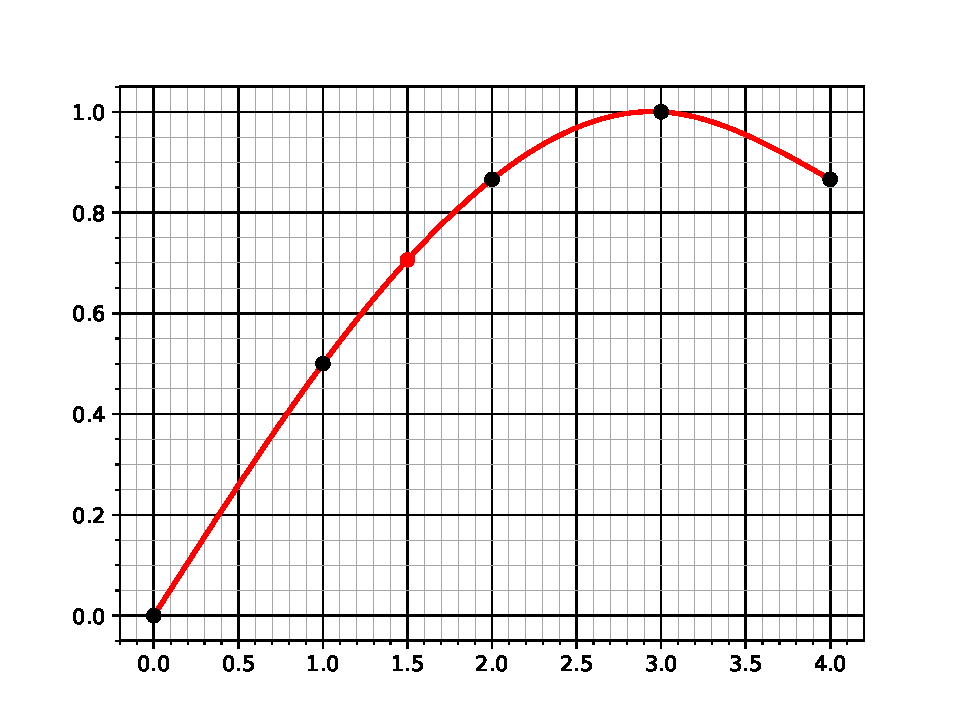
\includegraphics[width=\linewidth]{Pictures/1}
				\caption{График для пункта а)}
			\end{figure}
		
			Красной точкой отмечена точка интерполяции. 
			
			Из графика $f(x^*) = 0.7061482812500001$.
			
			
			\newpage
			
			\item[б)] Дана точка $x^* = 0.8$.
			\begin{table}[h!]
				\centering
				\begin{tabular}{|c|c|c|c|c|c|}
					\hline
					$x$    & $0.00000$ & $0.50000$ & $0.90000$ & $1.30000$ & $1.70000$ \\ \hline
					$f(x)$ & $-2.30260$ & $-0.69315$ & $-0.10536$ & $0.26236$ & $0.53063$ \\ \hline
				\end{tabular}
				\caption{Данные пункта б)}
			\end{table}
			
			Строим сплайн. Получаем график:
			\begin{figure}[h!]
				\centering
				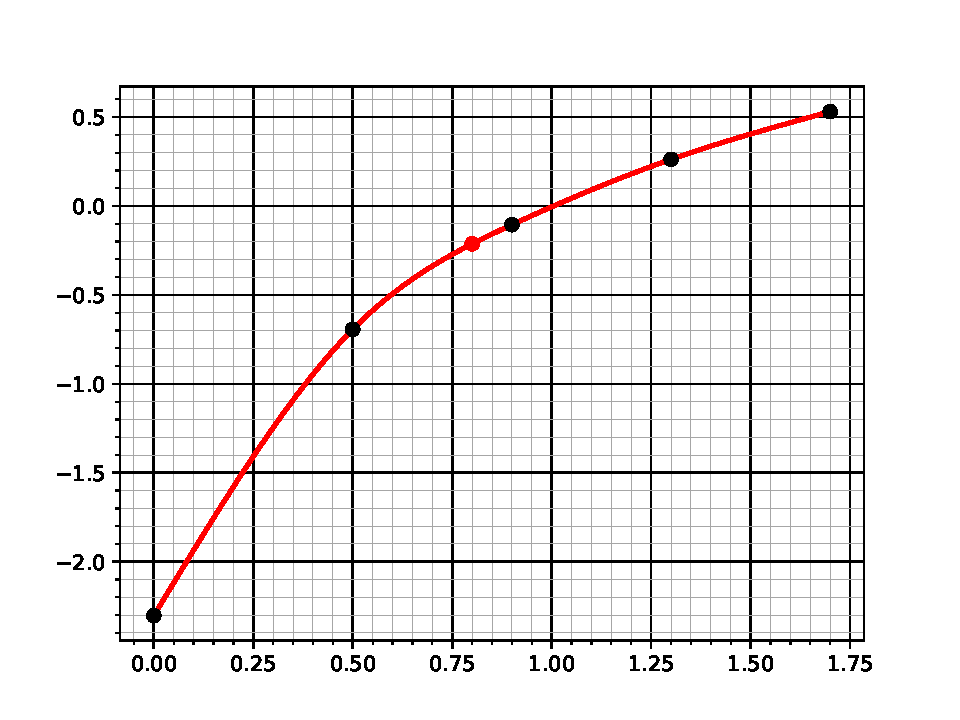
\includegraphics[width=\linewidth]{Pictures/2}
				\caption{График для пункта б)}
			\end{figure}
		
			Красной точкой отмечена точка интерполяции. 
			
			Из графика $f(x^*) = -0.21275445989173225$.
			
			
			
			\newpage
			
			\item[в)] Дана точка $x^* = 3.0$.
			\begin{table}[h!]
				\centering
				\begin{tabular}{|c|c|c|c|c|c|}
					\hline
					$x$    & $0.00000$ & $1.70000$ & $3.40000$ & $5.10000$ & $6.80000$ \\ \hline
					$f(x)$ & $0.00000$ & $1.30380$ & $1.84390$ & $2.25830$ & $2.60770$ \\ \hline
				\end{tabular}
				\caption{Данные пункта в)}
			\end{table}
			
			Строим сплайн. Получаем график:
			\begin{figure}[h!]
				\centering
				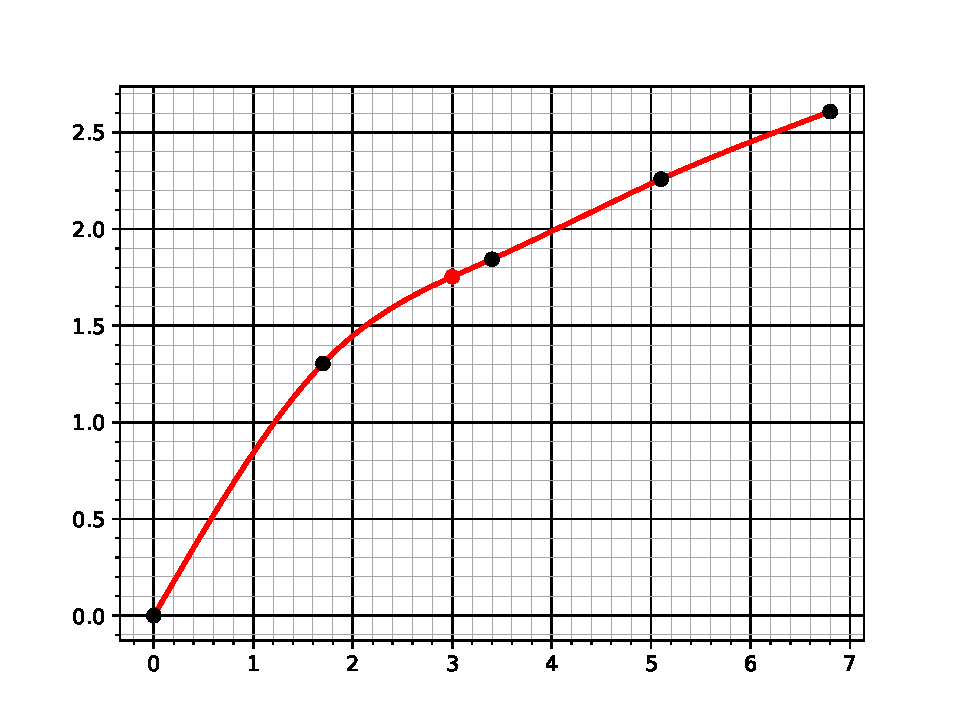
\includegraphics[width=\linewidth]{Pictures/3}
				\caption{График для пункта в)}
			\end{figure}
		
			Красной точкой отмечена точка интерполяции. 
			
			Из графика $f(x^*) = 1.7531560510017157$.
			
			
			
			
			\newpage
			
			\item[г)] Дана точка $x^* = 0.1$.
			\begin{table}[h!]
				\centering
				\begin{tabular}{|c|c|c|c|c|c|}
					\hline
					$x$    & $-0.40000$ & $-0.10000$ & $0.20000$ & $0.50000$ & $0.80000$ \\ \hline
					$f(x)$ & $1.98230$ & $1.67100$ & $1.36940$ & $1.04720$ & $0.64350$ \\ \hline
				\end{tabular}
				\caption{Данные пункта г)}
			\end{table}
			
			Строим сплайн. Получаем график:
			\begin{figure}[h!]
				\centering
				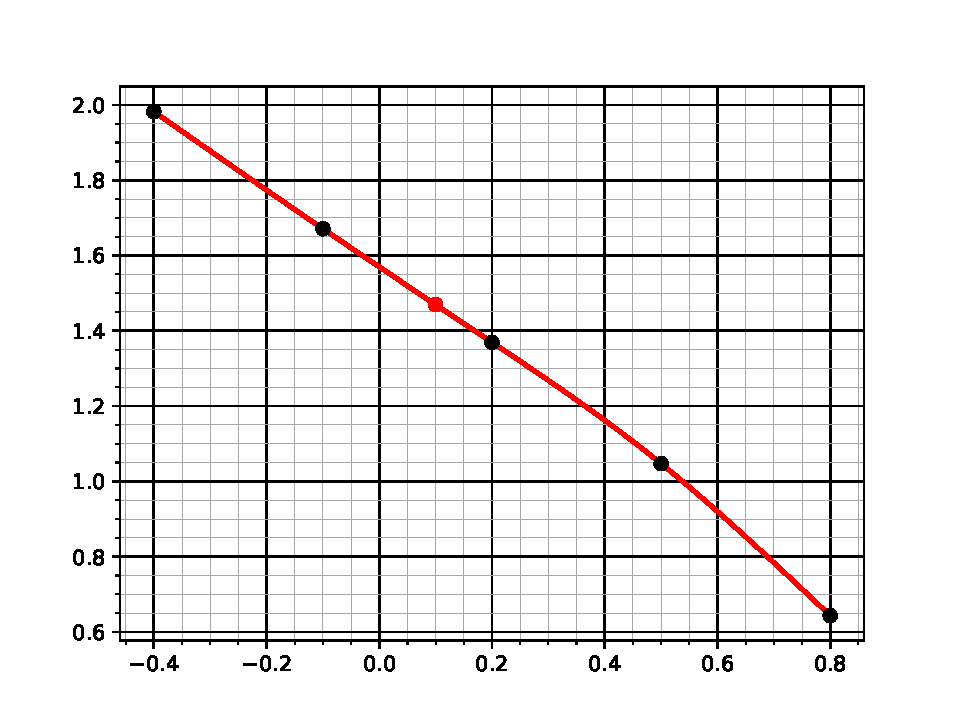
\includegraphics[width=\linewidth]{Pictures/4}
				\caption{График для пункта г)}
			\end{figure}
			
			Красной точкой отмечена точка интерполяции. 
			
			Из графика $f(x^*) = 1.4694391534391535$.
			
			
			\newpage
			
			\item[д)] Дана точка $x^* = 1.5$.
			\begin{table}[h!]
				\centering
				\begin{tabular}{|c|c|c|c|c|c|}
					\hline
					$x$    & $0.00000$ & $1.00000$ & $2.00000$ & $3.00000$ & $4.00000$ \\ \hline
					$f(x)$ & $1.00000$ & $1.54030$ & $1.58390$ & $2.01000$ & $3.34640$ \\ \hline
				\end{tabular}
				\caption{Данные пункта д)}
			\end{table}
			
			Строим сплайн. Получаем график:
			\begin{figure}[h!]
				\centering
				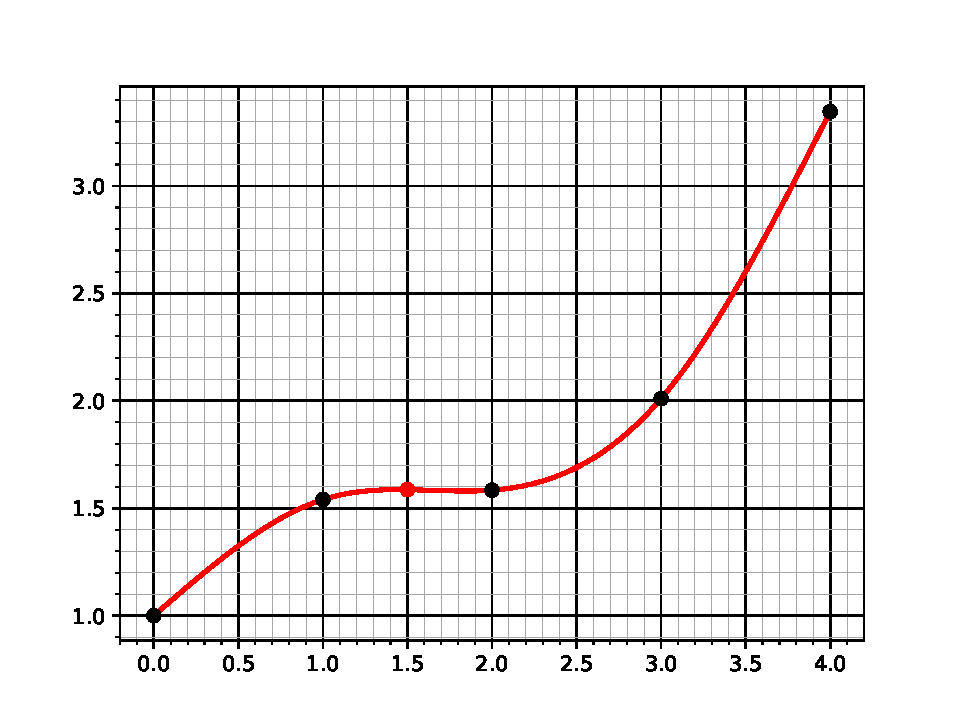
\includegraphics[width=\linewidth]{Pictures/5}
				\caption{График для пункта д)}
			\end{figure}
			
			Красной точкой отмечена точка интерполяции. 
			
			Из графика $f(x^*) = 1.5862379464285716$.
		\end{enumerate}
	
		Как видим, интерполяция удачна, ошибки малы.
		
		\newpage
		\tocsection{Оценка численности населения США}
		\tocsubsection{Общая постановка задачи}
		Для примера построения многочлена Ньютона и сплайн-интерполяции был взят номер \textbf{VI.9.32}. В нем таблично заданы значения численности населения США в период 1910--2000 гг. Наша задача -- экстраполировать зависимость к 2010 году.
		
		\begin{table}[h!]
			\centering
				\begin{tabular}{|c|r|}
					\hline
					Год  & \multicolumn{1}{c|}{Население} \\ \hline
					1910 & 92 228 496                                 \\ \hline
					1920 & 106 021 537                                \\ \hline
					1930 & 123 202 624                                \\ \hline
					1940 & 132 164 569                                \\ \hline
					1950 & 151 325 798                                \\ \hline
					1960 & 179 323 175                                \\ \hline
					1970 & 203 211 926                                \\ \hline
					1980 & 226 545 805                                \\ \hline
					1990 & 248 709 873                                \\ \hline
					2000 & 281 421 906                                \\ \hline
				\end{tabular}
			\caption{Тенденция численности населения США в период 1910--2000 гг.}
		\end{table}
	
		\newpage
		\tocsubsection{Интерполяция многочленом Ньютона}
		Для начала построим интерполянт в форме многочлена Ньютона. Алгоритм построения уже был описан в работе, поэтому просто предоставляем результаты.
	
		\begin{figure}[h!]
			\centering
			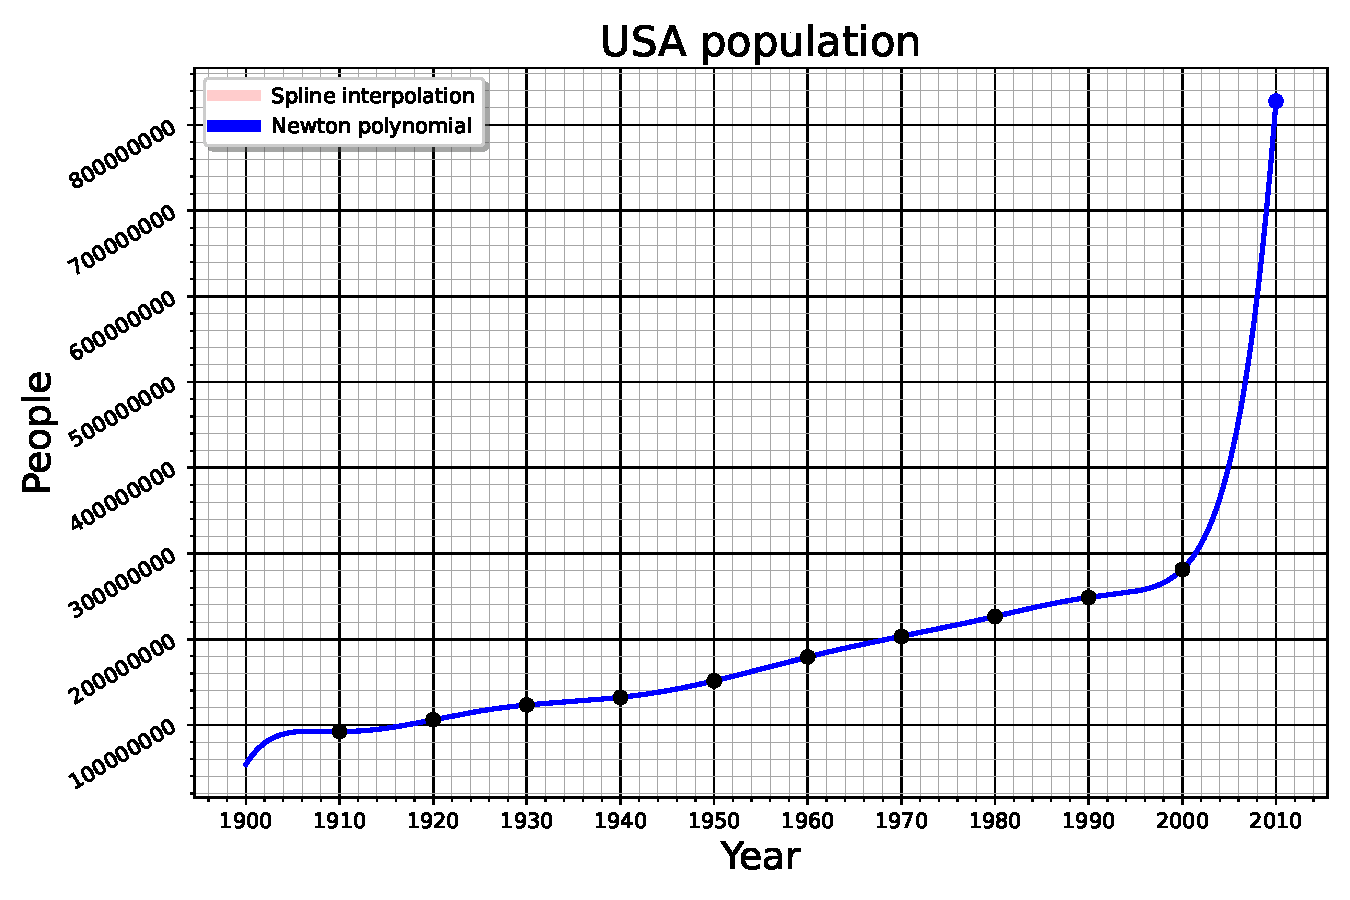
\includegraphics[width=\linewidth]{Pictures/Newton.pdf}
			\caption{Интерполяция многочленом Ньютона}
		\end{figure}
	
		По графику видно, что интерполяция удачна и весьма правдоподобна, чего нельзя сказать про необходимую экстраполяцию. На графике наблюдается резкий всплеск, предсказанная численность в 2010 году составляет 827 906 509 человек. В реальности такого скачка нет, и действительное значение населения 308 745 538 человек.
		
		Как видим, метод интерполяции многочленом Ньютона имеет колоссальную ошибку при экстраполяции. В данном случае она даже превосходит само действительное значение экстраполируемой величины.
	
		
		\newpage
		\tocsubsection{Сплайн-интерполяция}
		Теперь попробуем другой метод и выясним, какой же лучше. В этот раз построим кубический сплайн, причем будем использовать так называемый естественный сплайн. Опять же, весь алгоритм построения сплайна был описан выше, поэтому обсуждаем лишь результаты.
		\begin{figure}[h!]
			\centering
			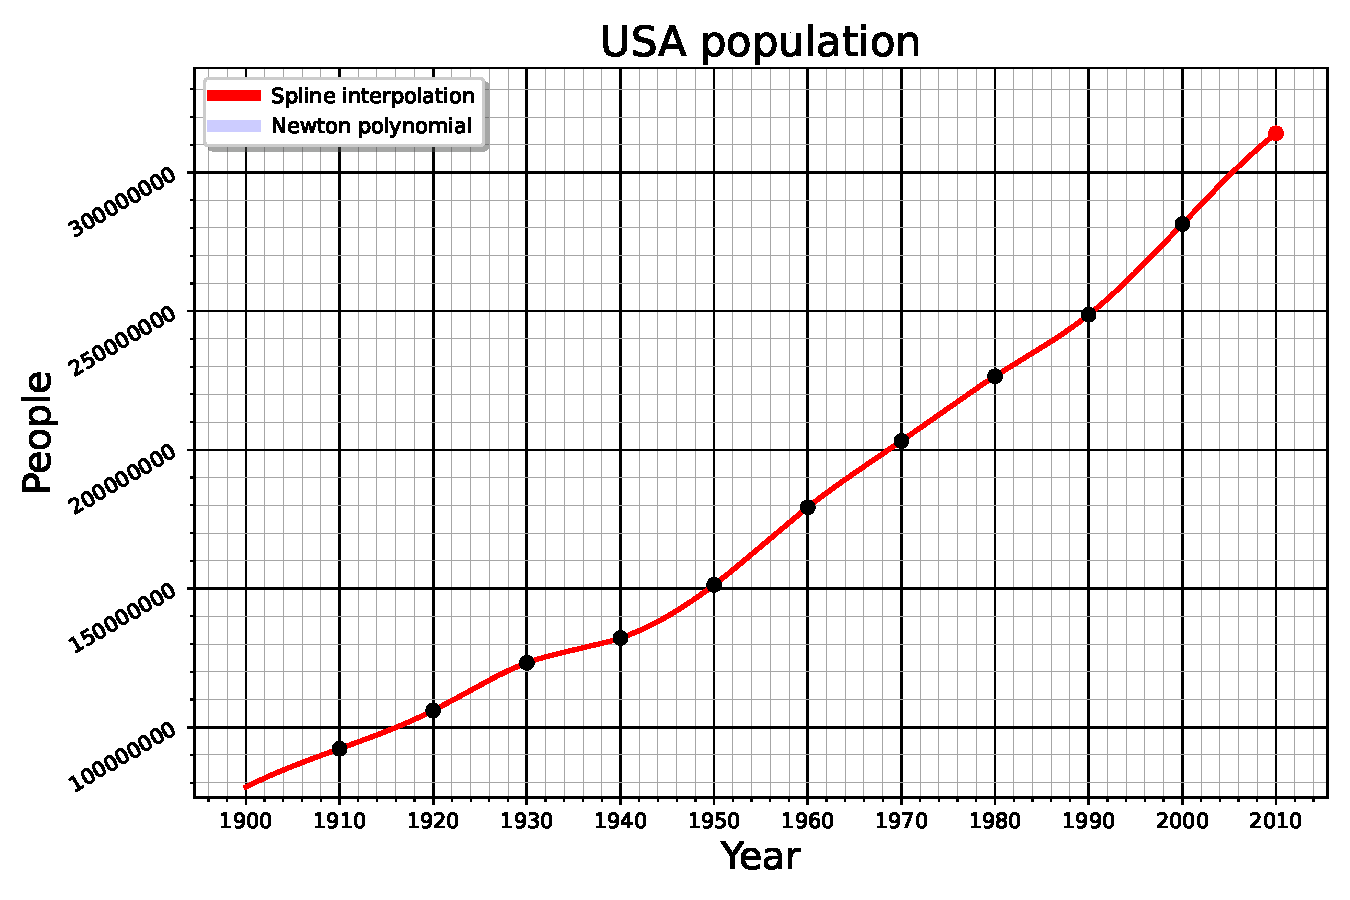
\includegraphics[width=\linewidth]{Pictures/Spline.pdf}
			\caption{Сплайн-интерполяция}
		\end{figure}
	
		Опять же, интерполяция более чем удачна. Однако на этот раз не только она, но и экстраполяция тоже. Предсказанное значение населения США к 2010 году составляет 314 133 939 человек. Это невероятно близко к настоящему значению 308 745 538! Ошибка составляет около $2\%$.
		
		\newpage
		
		\tocsection{Вывод}
		В данной работе были исследованы методы интерполяции такие как многочлен Ньютона и сплайн-интерполяция. По заданию с предсказанием населения США можно судить об их достоинствах и недостатках и провести сравнение методов между собой. В течение написания кода и тестирования программы было выяснено, что метод интерполяции многочленом Ньютона достаточно быстро и легко строится, однако имеет весомые ошибки при экстраполяции, хоть и при интерполяции они малы. У другого же метода --- сплайна --- ошибки малы как при интерполяции, так и при экстраполяции, но в противовес этому его достаточно трудоемко строить.
		
		Наиболее точную оценку населения США к 2010 году дал метод сплайн-интерполяции. Его предсказание -- 314 133 939 человек, что хорошо согласуется с действительным значением 308 745 538 с относительной ошибкой примерно $2\%$.
		
\end{document}